\documentclass{article}

\usepackage{fullpage,amsmath,amsthm,graphicx,enumitem}
\usepackage{hyperref}
\usepackage{amssymb}
\usepackage{wasysym}
\usepackage{color}
\usepackage[capitalize]{cleveref}
\usepackage{xurl}

\newcommand{\todo}[1]{\textbf{\textcolor{red}{#1}}}

\theoremstyle{definition}
\newtheorem{task}{Task}
\crefname{task}{Task}{Tasks}

\newcommand{\option}{{\Large$\Square$ }}

\title{ASEN 3728 Aircraft Dynamics\\Programming Homework 3}

\date{Due date listed on Gradescope.}

\begin{document}

\maketitle

In this assignment, you will create a nonlinear model of a conventional aircraft, simulate its longitudinal motion, and compare the results with a linear approximation.
The aircraft is the TTwistor, a twin engine research aircraft designed here at CU Boulder and pictured below. The aircraft parameters are given in the Matlab struct returned by the \texttt{ttwistor} function.

\begin{center}
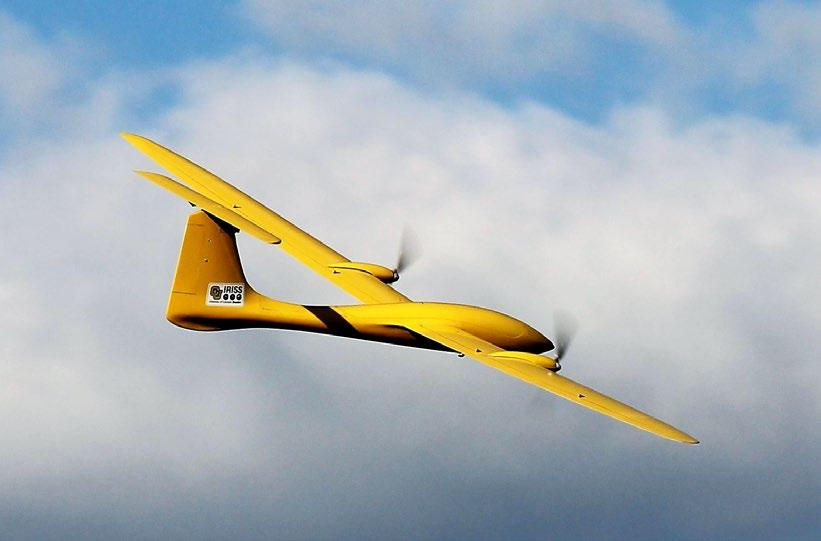
\includegraphics[width=3in]{ttwistor.jpg}
\end{center}

All files are available by cloning the git repository at \url{https://github.com/zsunberg/Aircraft-Dynamics-Materials} and navigating to the \texttt{assignments/P3} directory. A zip file is also available at \url{https://github.com/zsunberg/Aircraft-Dynamics-Materials/raw/main/zips/assignments/P3.zip}. It is possible that there will be bugfixes to the assignment after it is released. These will be announced on Piazza.

\begin{task}
    Implement the \texttt{lonAeroForcesAndMoments} function and run the tests as indicated in \texttt{TEMPLATE\_report.m} to verify that it is implemented correctly. See the documentation of the function for details about inputs and outputs. You may look at \texttt{latAeroForcesAndMoments.m} to see a similar implementation for lateral dynamics.

    Assume that the lift and moment coefficients are linear functions of $\alpha$, $\hat{q}$, and $\delta_e$, and that $C_D = C_{D_\text{min}} + K (C_L - C_{L_\text{min}})^2$.Additionally, assume that all derivatives related to $\dot{\alpha}$ are zero. Use the thrust model already implemented in \texttt{TEMPLATE\_lonAeroForcesAndMoments.m} and assume that the thrust is aligned with the x axis of the aircraft. Note that the field \texttt{CL0} is the lift coefficient at zero angle of attack - not the lift coefficient at the minimum drag angle of attack or the lift coefficient at trim.
\end{task}

\begin{task}
    Implement the \texttt{aircraftDynamics} function and run the tests as indicated in \texttt{TEMPLATE\_report.m} to verify that it is implemented correctly. See the documentation of the function for details about inputs and outputs. Much of the code for this can be copied from the \texttt{monospinnerDynamics} function from assignment P1.
\end{task}

\begin{task}
    Run the \texttt{evaluate} function to produce a \texttt{submission.json} file that certifies that the tests pass for your implementations of \texttt{lonAeroForcesAndMoments} and \texttt{aircraftDynamics}.
\end{task}

\begin{task}
    Use the \texttt{estimateAlon} function to estimate $A_\text{lon}$ with the trim state and control settings in \texttt{TEMPLATE\_report.m}. Calculate the eigenvectors of the resulting $A_\text{lon}$ matrix and indicate which of the vectors correspond to the short period and phugoid modes.
\end{task}

\begin{task}
    Determine an initial state for the four-dimensional linear model with an initial pitch deviation of $\Delta\theta = 10^\circ$ that only excites the \emph{phugoid mode}.
    Use this initial deviation state and the trim state to determine a twelve-dimensional initial state for the nonlinear model that starts with the same pitch angle and minimizes short period oscillations.
    Simulate both the linear and nonlinear models for 50 seconds starting at these initial conditions and plot the pitch angle.
    Provide axis labels with units for the plots and indicate with a legend which are the linear and nonlinear results.
\end{task}

\begin{task}
    Determine an initial state for the four-dimensional linear model with an initial pitch deviation of $\Delta\theta = 10^\circ$ that only excites the \emph{short period mode}.
    Use this initial deviation state and the trim state to determine a twelve-dimensional initial state for the nonlinear model that starts with the same pitch angle and minimizes phugoid oscillations.
    Simulate both the linear and nonlinear models for 10 seconds starting at these initial conditions and plot the pitch angle.
    Provide axis labels with units for the plots and indicate with a legend which are the linear and nonlinear results.
\end{task}

\begin{task}
    Briefly explain the discrepancy between the linear and nonlinear simulation results for the initial condition designed to excite the short period mode.
\end{task}

\subsection*{Deliverables}
In order to use the template files, rename them by removing \texttt{TEMPLATE\_}. To produce the report with plots, using the Matlab command \texttt{publish('report.m', 'pdf')} is highly recommended. Submit the following files to Gradescope:

\begin{itemize}[noitemsep]
    \item \texttt{submission.json} (make sure that the Gradescope autograder runs successfully when you submit!)
    \item \texttt{report.pdf} containing required output from the tasks.
    \item \texttt{lonAeroForcesAndMoments.m}
    \item \texttt{aircraftDynamics.m}
    \item Any additional supporting functions you may have written.
\end{itemize}

\end{document}
